\section{Обзор предметной области}
\label{sec:domain:intro}

В данном разделе будет произведён обзор программных средств аналогичных разрабатываемому в рамках работы, а так же литературных источников. Проанализированы преимущества и недостатки различных подходов к выделению, обработке и классификации признаков рукописного текста.

\subsection{Биометрическая аутентификация}
\label{sub:domain:bioauthentication}
\emph{Биометрическая аутентификации} -- это распознавание объекта основано на сравнении физиологических или психологических особенностей этого объекта с его характеристиками, хранящимися в
базе данных системы.

Биометрические технологии можно разделить на две большие категории - физиологические и психологические (поведенческие). В первом случае анализируются такие признаки, как черты лица, структура глаза, параметры пальцев, ладонь, форма руки. Психологические характеристики - это голос человека, особенности его подписи, динамические параметры письма и особенности ввода текста с клавиатуры~\cite{bioauth_dinamic_moves}.
Логически биометрическую систему можно разделить на два модуля: модуль регистрации и модуль аутентификации.

На этапе регистрации биометрические датчики сканируют необходимые физиологические или поведенческие характеристики человека и создают их цифровое представление. Специальный модуль обрабатывает это представление с целью выделить характерные особенности и сгенерировать эталон. На этапе аутентификации биометрический датчик снимает характеристики человека, которого нужно аутентифицировать, и преобразует эти характеристики в тот же цифровой формат, в котором хранится эталон. Полученный набор характеристик сравнивается с хранимым, чтобы определить, соответствуют ли они друг другу.

\todo[inline]{Вычитать, Вставить ссылки}
\subsubsection{Методы биометрической аутентификации}
Методы биометрической аутентификации можно разделить на две группы~\cite{wiki_sign_verification}:

Статические методы -- основываются на физиологической (статической) характеристике человека, то есть уникальной характеристике неотъемлемых от него.
Примерами статических методов являются:
\begin{itemize}
  \item по отпечатку пальца (В основе этого метода лежит уникальность рисунка папиллярных узоров на пальцах);
  \item по форме ладони (С помощью специального устройства строится трехмерный образ кисти);
  \item по форме лица. (На лице выделяются контуры бровей, глаз, носа, губ и т.д., вычисляется расстояние между ними и строится не просто образ, а еще множество его вариантов на случаи поворота лица, наклона, изменения выражения);
  \item по сетчатке глаза;
  \item по радужной оболочке глаза;
  \item по ДНК.
\end{itemize}

Динамические методы -- основываются на поведенческой (динамической) характеристике человека, то есть построены на особенностях, характерных для подсознательных движений в процессе воспроизведения какого-либо действия.
Примерами динамических методов являются:
\begin{itemize}
  \item по рукописному почерку (росписи);
  \item по клавиатурному почерку (набор кодового слова);
  \item по голосу (частотных и статистических характеристик звука).
\end{itemize}
Сравнивать описанные выше биометрические методы по показаниям ошибок первого рода (не пустить в систему «своего») очень сложно, так как они сильно разнятся из-за сильной зависимости от оборудования на котором они реализованы~\cite{lorette_plamondon}.

По показателям ошибок второго рода (пустить в систему чужого) общая сортировка методов биометрической аутентификации выглядит так (от лучших к худшим):
\begin{enumerate}
  \item ДНК;
  \item радужная оболочка глаза, сетчатка глаза;
  \item отпечаток пальца, термография лица, форма ладони;
  \item форма лица, расположение вен на кисти руки и ладони;
  \item подпись;
  \item клавиатурный почерк;
  \item голос.
\end{enumerate}

При современном уровне развития технологий, с каждым днем растет количество пользовательских данных доступных через глобальную сеть, электронную почту, файловые хранилища, различные облачные сервисы. В связи с этим вопрос надежности процедуры аутентификации стоит, как никогда остро. Однако увеличивающееся число аутентификаций, которое должен проходить пользователь ежедневно, приводит к новым проблемам. Упрощение процедуры аутентификации для конечного пользователя, при этом сохранение ее надежности, является перспективным направлением исследований.

\todo[inline]{Вычитать}
\todo[inline]{Добавить источники}
\subsection{Микрография}
\emph{Микрография} - это приобретенное расстройство, которое характеризуется аномально малым, стесненным почерком или прогрессией до постепенному уменьшению почерка.~\cite{larner_dict_neuro} Он обычно ассоциируется с нейродегенеративными нарушениями базальных ганглий, такими как болезнь Паркинсона, но также приписывается подкорковым очагам поражения~\cite{academic_press_movement_disorders}. О'Салливан и Шмитц описывают его как ненормально маленький почерк, который трудно читать.~\cite{o_sullivan} Микрография также наблюдается у пациентов с болезнью Вильсона, обсессивно-компульсивным расстройством, метаморфопсией или с изолированными очаговыми поражениями среднего мозга или базальных ганглий.~\cite{kinematic_hardwrittung_analysis}

Неврологические заболевания такие как болезнь Паркинсона, синдром дефицита внимания и гиперактивности могут быть диагностированы на начальных стадиях на основе анализа параметров почерка либо динамики изменения параметром. Данные подход позволяет удешевить и ускорить первичную диагностику неврологические заболеваний.
При анализе почерка пациентов страдающих неврологическими заболеваниями было выяснено что у 7 - 95\% появляются в различной степени микрография и нечеткость контуров символов вызванная тремором. Микрография - это приобретенное расстройство, характеризующие аномально малым, стесненным почерком или прогрессирующим уменьшением почерка.

Оба критерия хорошо поддаются автоматическому выделению и оценке. Так для текущего состояния и динамики развития микрографии достаточно несколько образцов почерка на листах одного или схожего размера, например A4, однако наличие линейной сетки на листе позволит получить более точные данные.
Для анализа второго фактора в качестве меры может быть принято отклонение элемента рукописного символа от его скелета. Сумма отклонений деленная на общее число выделенных элементов принимается за текущий показатель.
Существуют так же и другие параметры опущенные в данной статье виду большей сложности расчета и автоматизации, а так меньшей корреляциею с неврологическими заболеваниями, например сила нажатия и количество ошибок.

Учитывая индивидуальные особенности почерка отдельного человека и погрешности при оцифровке, если сбор образца производился не в цифровом виде, приводит к существенного разбросу параметров от человеку к человеку что делает невозможным выявление небольших отклонений без анализ динамики.
Анализируя выше изложенный набор факторов можно повысить эффективность более дорогостоящих и долгих исследований и анализов.
Описанный подход является эффективным, однако он может выявлять неврологические заболеваниях на ранних стадиях только при анализу динамики изменения параметров, что требует накопления информации об отдельном пациенте.

\subsection{Графология}
\label{sub:domain:grafologic}
\emph{Графология} -- это учение, постулирующее наличие устойчивой связи месту почерком и индивидуальными особенностями личности.

Идея использования почерка для выявления психологических параметров личности впервые была предложена в 1622 в книге итальянского профессора Камилло Бальдо <<Как узнать природу и качества человека, взглянув на букву, которую он написал>>~\cite{kamillo_grafology}. Первым кто систематизировал знания стал Фландрэна аббат Мишон в 1872 году. Он проанализировал большое количество работ по графологии и образцов почерка и в своей книге <<Система графологии>> предложил \emph{метод Мишона}, он основывался на анализе штрихов, букв, слов, свободных движений, строк и пр.~\cite{mishon_grafology}

Начиная с середины 20-го века графология начала рассматриваться как псевдонаучное учение~\cite{graphology_wiki}. По результатам исследования профессиональным графологам не удалось достоверно оценить трудовые способности человека. В среднем профессиональные графологи давали такую же по степени достоверности оценку, как и люди «с улицы»~\cite{neter_shakhar_psevdograph, king_koehler_psevdograph}. В десятках исследований было показано отсутствие связи особенностей почерка с трудовыми способностями человека.

Тем не менее графология широко используется в современной практике отбора кадров~\cite{graphology_psyfactor}.

Основные признаки почерка, которые анализирует графологическая экспертиза:
\begin{enumerate}
  \item размер букв (очень маленькие, маленькие, средние, крупные);
  \item наклон букв (левый наклон, легкий наклон влево, правый наклон, резкий наклон вправо);
  \item направление почерка: (строчки ползут вверх, строчки прямые, строчки ползут вниз);
  \item размашистость и сила нажима: (легкая, средняя, сильная, очень сильная);
  \item характер написания слов (склонность к соединению букв и слов, склонность к отдалению букв друг от друга, смешанный стиль);
  \item общая оценка (почерк старательный, почерк неровный, почерк небрежный, почерк неразборчивый).
\end{enumerate}

Перечисленные параметры почерка являются устойчивыми, но все же присутствует естественные отклонения параметров (длина, ширина, толщина, угол) от средних значений. Вариация становится наиболее заметной при изменение психологического состояния человека, например при страхе, беспокойстве, алкогольном опьянении.

\subsection{Анализ аналогов}
\label{sub:domain:analogs}

\todo[inline]{нужно лишь сделать акцент на медицину}
\subsubsection{MovAlyzeR}
\label{sub:domain:analogs:movalyzer}
Программное средство <<MovAlyzeR>> является частью семейства программных средств для работы с рукописным текстов компании <<NeuroScript>> и представляет собой десктопное приложение для операционных систем Windows~\cite{analogs_movalyzer}. Пользовательский интерфейс приложения представлен на рисунке~\ref{fig:domain:analogs:movalyzer}.
Основными возможностями ПС являются:
\begin{itemize}
  \item отслеживание положения, давления, ориентации с частотой \mbox{100-200 Гц;}
  \item поддержка отслеживания руки, стилуса и мыши;
  \item измерение координации обеих рук одновременно;
  \item отображение результатов в реальном времени;
  \item изменение толщины линии, визуальная и звуковая обратная связь;
  \item искажение визуальная обратная связь, поворот, перекос и отражение на мониторе компьютера в режиме реального времени;
  \item моделирование, генерация рукописных цифровых данных с шумом и известными характеристиками штрихов;
  \item проверка непротиворечивости;
  \item анализ результатов, статистика результатов с визуализацией;
  \item многостраничная запись, разделение текст на слова и штрихи;
  \item внешние приложения, полная интеграция с вашими собственными модулями с использованием сценариев MATLAB или скомпилированных программ;
  \item оптически сканированные изображения.
\end{itemize}

Основными недостатками ПС являются:
\begin{itemize}
  \item поддержка только ОС семейства Windows (XP, 7, 8);
  \item платное использование (799+ \$).
\end{itemize}

ПС может быть использовано для оценки моторных функций и диагностики неврологических отклонений.

\begin{figure}[ht]
    \centering
    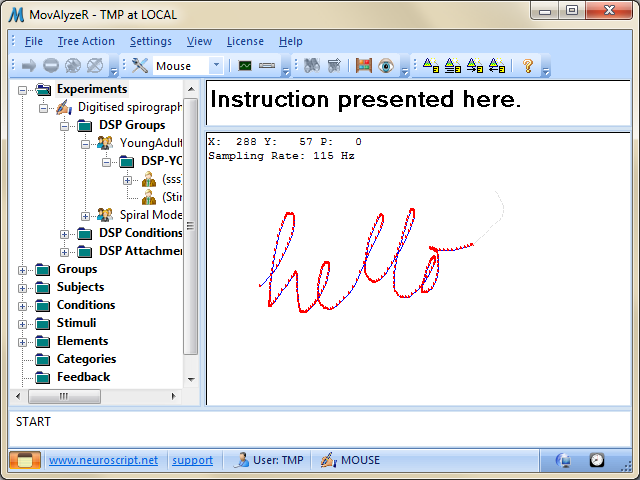
\includegraphics[width=0.7\textwidth]{figures/movalyzer.png}
    \caption{Программное средство <<Movalyzer>>}
    \label{fig:domain:analogs:movalyzer}
\end{figure}

В настоящий момент существует достаточное количество исследований, часть из них будет рассмотрена в разделе~\ref{sub:domain:literary_sources}, доказывающих связь отклонений к почерке с развитием неврологических заболеваний, однако на рынке представлено относительно небольшое количество аналогов ввиду дороговизны разработки ПО в сфере здравоохранения и ряда этических вопросов связанных со сбором и обработкой историй болезни.

\subsubsection{Web-Key}
\label{sub:domain:analogs:biokey}
Семейство программных и технических средств компании <<Bio-Key>>~\cite{analogs_biokey} предназначено для внедрения аутентификации на основе отпечатков пальце в корпоративные системы. Далее будет рассмотрено программное средство <<Web-Key>> как наиболее близкое по функционалу к рассматриваемому в работе.

\todo{Вычитать}
Основными возможностями и достоинствами ПС являются:
\begin{itemize}
  \item точная и быстрая аутентификация пользователей на предприятии;
  \item высочайшие результаты независимой проверки и проверки NIST по скорости и точности аутентификации на основе отпечатков пальцев;
  \item возможность использования отдельно, совместно с паролями или другими способами аутентификации для гибкости в развертывании;
  \item поддержка Plug-and-Play (включая Windows Biometric Framework) для считывателей отпечатков пальцев от всех основных производителей;
  \item пошаговая аутентификация для доступа к определенным модулям или данным или для завершения определенных конфиденциальных транзакций;
  \item механизм векторной сегментации (VST) BIO-key предназначен для сопоставления «один ко многим» с группами пользователей практически любого размера;
  \item сервер аутентификации может быть развернут в общедоступном или частном облаке для дополнительной масштабируемости и снижения требований к ИТ-ресурсам компании;
  \item шифрование на основе PKI защищает все данные, передаваемые между компонентами ПС;
  \item многоуровневое тройное шифрование самих моделей отпечатков пальцев для предотвращения мошеннического захвата данных;
  \item решение основанные на отпечатках пальцев намного дешевле, чем другие биометрические решения, такие как сканирование радужной оболочки глаза, для которых требуется специализированное оборудование в каждой точке входа.
\end{itemize}

Основными недостатками ПС являются:
\begin{itemize}
  \item необходимость использования специального оборудования;
  \item дорогостоящая лицензия.
\end{itemize}

\subsubsection{BioID Web-Service}
\label{sub:domain:analogs:bioId}
Семейство программных средств компании <<BioID>>~\cite{analogs_bioid} предназначено для аутентификации частных и корпоративных клиентов на основе формы лица. Далее будет рассмотрено программное средство <<BioID Web-Service>> как наиболее близкое по функционалу к рассматриваемому в работе.

\todo{Вычитать}
Основными возможностями и достоинствами ПС являются:
\begin{itemize}
  \item хорошо спроектированный SOAP или RESTful Web API;
  \item облачное решение, дата-центры по всему миру;
  \item прозрачная высокая масштабируемость с балансировщиком нагрузки;
  \item передача данных защищена шифрованием TLS / SSL;
  \item контроль доступа с помощью клиентских сертификатов X.509 (SOAP) или токена приложения (REST);
  \item изолированный экземпляр сервиса для каждого клиента;
  \item запатентованная антиспуфинговая технология обнаружения фотографий и видео для предотвращения мошенничества и нелегального доступа.
\end{itemize}

Основными недостатками ПС являются:
\begin{itemize}
  \item необходимость использования специального оборудования;
  \item дорогостоящая лицензия.
\end{itemize}

\subsubsection{Aware WebEnroll}
\label{sub:domain:analogs:aware}
Семейство программных средств компании <<Aware>>~\cite{analogs_aware} предназначено для аутентификации корпоративных клиентов на основе широкого набора методов, таких как отпечаток пальца, форма лица, сетчатка глаза, голос и другие. Далее будет рассмотрено программное средство <<WebEnroll> как наиболее близкое по функционалу к рассматриваемому в работе.

\todo{Вычитать}
Основными возможностями и достоинствами ПС являются:
\begin{itemize}
    \item поиск, сортировка и фильтрация транзакций;
    \item создание пользователей и групп;
    \item поддержка ролевой модели доступа;
    \item предотвращение повторного использования паролей;
    \item принудительная смена пароля через указанное количество дней;
    \item блокировка аккаунта после указанного количества неудачных входов в систему в течение указанного интервала времени;
    \item блокировка аккаунта через указанное количество дней бездействия.
\end{itemize}

Основными недостатками ПС являются:
\begin{itemize}
  \item необходимость использования специального оборудования;
  \item дорогостоящая лицензия.
\end{itemize}

\subsubsection{Bio-IDiom}
\label{sub:domain:analogs:nec}
Семейство программных средств в области биометрической аутентификации компании <<NEC>>~\cite{analogs_nec} предназначено для повышения уровня безопасности и уменьшения риска несанкционированного доступа к ресурсам корпоративных клиентов на основе широкого набора методов, таких как отпечаток ладони, рисунок капилляров, сетчатка глаза, голос и другие. Далее будет рассмотрено программное средство <<Bio-IDiom> как наиболее близкое по функционалу к рассматриваемому в работе.

\todo{Вычитать}
Основными возможностями и достоинствами ПС являются:
\begin{itemize}
  \item широкий спектр поддерживаемых способов аутентификации;
  \item возможность использования многофакторной аутентификации.
\end{itemize}

Основными недостатками ПС являются:
\begin{itemize}
  \item необходимость использования специального оборудования;
  \item дорогостоящая лицензия.
\end{itemize}

На рынке представлен широкий набор программных и аппаратных средств биометрической аутентификации, как для частных, так и для корпоративных клиентов и высокой степенью точности и отказоустойчивости, однако все они отличаются высокой стоимостью лицензии и зачастую требуют использования дорогостоящего оборудования~\cite{wacom_lcd}.

\subsubsection{ScriptAlyzeR}
\label{sub:domain:analogs:neuro_script}
Программное средство <<ScriptAlyzeR>> является частью семейства программных средств для работы с рукописным текстов компании <<NeuroScript>> и представляет собой десктопное приложение для операционных систем Windows~\cite{analogs_scriptAlyzer}. Пользовательский интерфейс приложения представлен на рисунке~\ref{fig:domain:analogs:neuro_script}. Программное средство использует одно функциональное ядро с ранее рассмотренным <<MovAlyzeR>>~\ref{sub:domain:analogs:movalyzer}, однако имеет отличную область применения.

Основными возможностями ПС являются:
\begin{itemize}
  \item отслеживание положения, давления, ориентации с частотой \mbox{100-200 Гц;}
	\item поддержка отслеживания руки, стилуса и мыши;
	\item измерение координации обеих рук одновременно;
	\item отображение результатов в реальном времени;
	\item изменение толщины линии, визуальная и звуковая обратная связь;
	\item искажение визуальная обратная связь, поворот, перекос и отражение на мониторе компьютера в режиме реального времени;
	\item моделирование, генерация рукописных цифровых данных с шумом и известными характеристиками штрихов;
	\item проверка непротиворечивости;
	\item анализ результатов, статистика результатов с визуализацией;
	\item многостраничная запись, разделение текст на слова и штрихи;
	\item внешние приложения, полная интеграция с вашими собственными модулями с использованием сценариев MATLAB или скомпилированных программ;
	\item оптически сканированные изображения.
\end{itemize}

Основными недостатками ПС являются:
\begin{itemize}
  \item поддержка только ОС семейства Windows (XP, 7, 8);
  \item платное использование (799+ \$).
\end{itemize}

Согласно утверждениям разработчиков ПС может быть использовано для оценки моторных функций, а так же тестирования на состояние алкогольного опьянения.

\begin{figure}[ht]
    \centering
    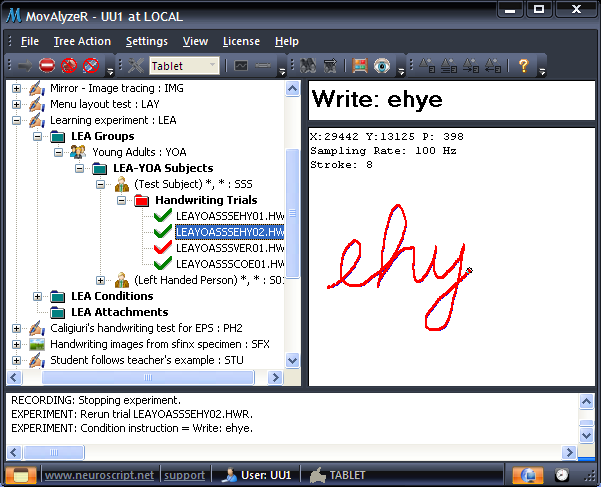
\includegraphics[width=0.7\textwidth]{figures/neuroscript.png}
    \caption{Программное средство <<ScriptAlyzeR>>}
    \label{fig:domain:analogs:neuro_script}
\end{figure}

\subsubsection{Graphology}
\label{sub:domain:analogs:graphology}
Программное средство <<Graphology>> является приложением для операционной системы Android, разработанным компанией <<LH Apps>>~\cite{analogs_graphology}.

Программное средство <<Graphology>> предназначено для анализа почерка и определения характеристик личности. Алгоритм работы программы основан на обширных исследованиях и был создан при консультации профессиональных экспертов графологии. Пользовательский интерфейс приложения представлен на рисунке~\ref{fig:domain:analogs:graphology}.

Основными возможностями ПС являются:
\begin{itemize}
  \item поддержка ОС Android;
  \item многофакторная оценка параметров личности (почерк, подпись);
  \item выполнение анализа без доступа в интернет.
\end{itemize}

Основными недостатками ПС являются:
\begin{itemize}
  \item поддержка только ОС Android;
  \item поддержка только английского языка;
  \item для ввода образцов почерка используется экран смартфона, что приводит к искажению в написании символов при низком разрешении и без использование стилуса.
\end{itemize}

\begin{figure}[ht]
    \centering
    
\includegraphics[width=0.7\textwidth]{figures/graphology_analog.jpeg}
    \caption{Программное средство <<Graphology>>}
    \label{fig:domain:analogs:graphology}
\end{figure}

\subsubsection{Signature Analysis}
\label{sub:domain:analogs:signature_analysis}

Программное средство <<Signature Analysis>> является приложением для операционной системы Android, разработанным компанией <<Beyond Consultancy Services>>~\cite{analogs_signature_analysis}.

Программное средство <<Signature Analysis>> предназначено для определения характеристик личности по образцу подписи. В разработке участвовал графолог с многолетним опытом, выступающей в качестве консультанта многих крупных компаний.  Пользовательский интерфейс приложения представлен на рисунке~\ref{fig:domain:analogs:signature_analysis}.

Основными возможностями ПС являются:
\begin{itemize}
  \item поддержка ОС Android;
  \item широкий спектр анализируемых параметров подписи (скорость, давление, длины, направления);
\end{itemize}

Основными недостатками ПС являются:
\begin{itemize}
  \item поддержка только ОС Android;
  \item платный анализ каждой подписи (0,83 \$);
  \item для работы необходимо интернет соединение;
  \item для ввода образцов почерка используется экран смартфона, что приводит к искажению в написании символов при низком разрешении и без использование стилуса.
\end{itemize}

\begin{figure}[ht]{}
    \centering
    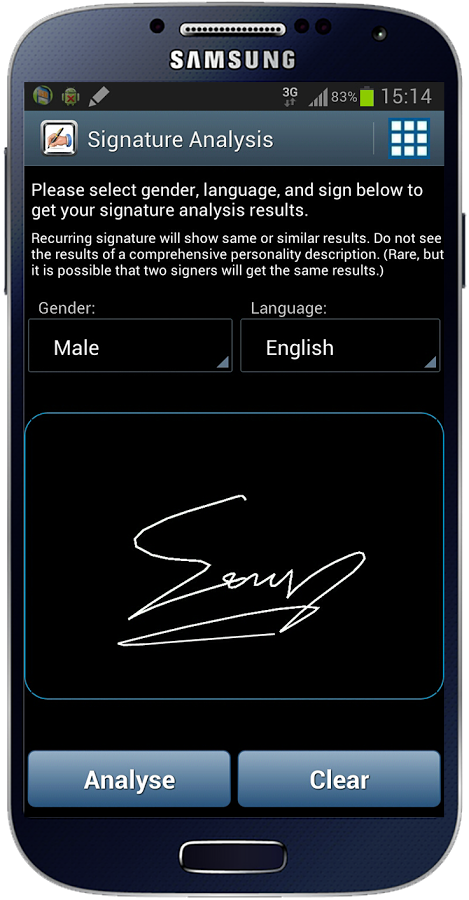
\includegraphics[height=0.4\textheight]{figures/analog_signature_analysis.png}
    \caption{Программное средство <<Signature Analysis>>}
    \label{fig:domain:analogs:signature_analysis}
\end{figure}

\subsubsection{My Graphology}
\label{sub:domain:analogs:my_graphology}
Программное средство <<My Graphology>> является приложением для операционной системы Android, разработанным компанией <<PENS>>~\cite{analogs_my_graphology}. Пользовательский интерфейс приложения представлен на рисунке~\ref{fig:domain:analogs:my_graphology}.

\begin{figure}[h]
    \centering
    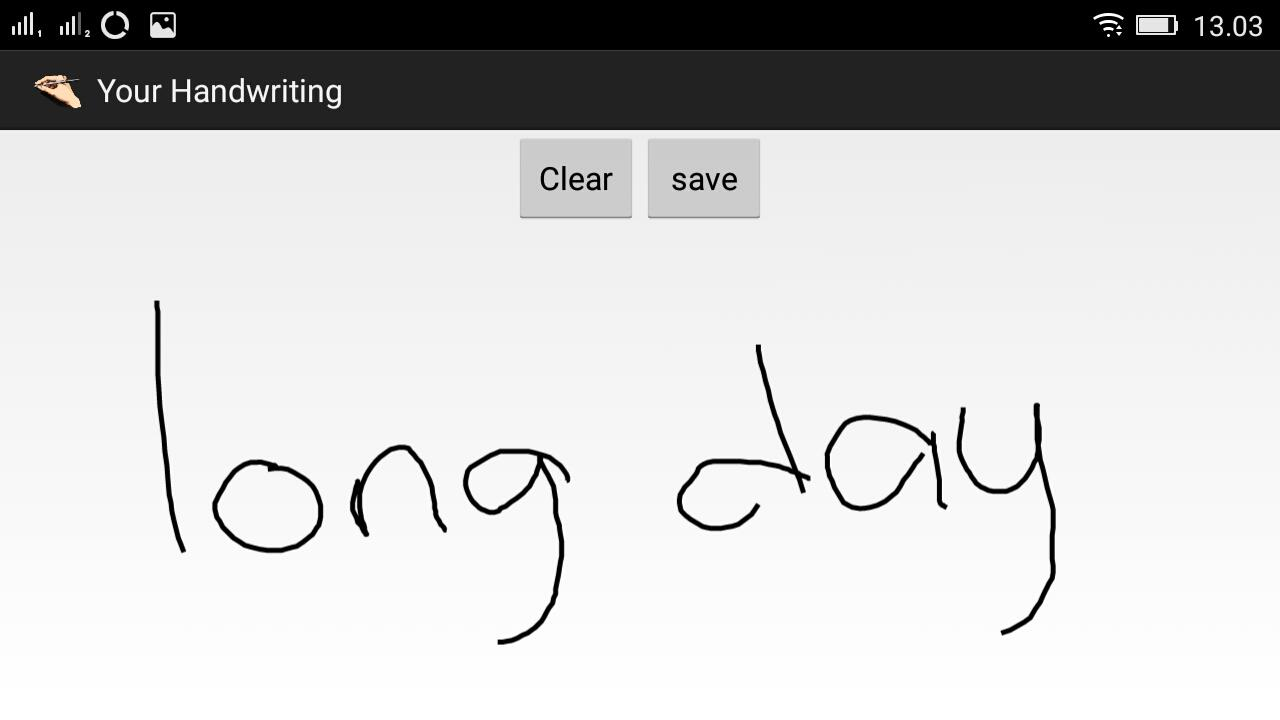
\includegraphics[width=0.4\textheight]{figures/analog_my_graphology.jpeg}
    \caption{Программное средство <<My Graphology>>}
    \label{fig:domain:analogs:my_graphology}
\end{figure}

Основными возможностями ПС являются:
\begin{itemize}
  \item поддержка ОС Android;
  \item использование для ввода экрана или фотографии почерка;
  \item выполнение анализа без доступа в интернет.
\end{itemize}

Основными недостатками ПС являются:
\begin{itemize}
  \item поддержка только ОС Android;
  \item в разработке не участвовали эксперты графологи;
  \item поддержка только испанского языка интерфейса.
\end{itemize}

\subsubsection{GRAPHOLOGY signature analysis}
\label{sub:domain:analogs:graphology_sign_analysis}
Программное средство <<GRAPHOLOGY signature analysis>> является приложением для операционной системы Android, разработанным компанией <<DokThor>>~\cite{analogs_graphology_sign_analysis}. Программное средство <<GRAPHOLOGY signature analysis>> предназначено для определения характеристик личности по образцу подписи. Пользовательский интерфейс приложения представлен на рисунке~\ref{fig:domain:analog:graphology_sign_analysis}.

\begin{figure}[h]
    \centering
    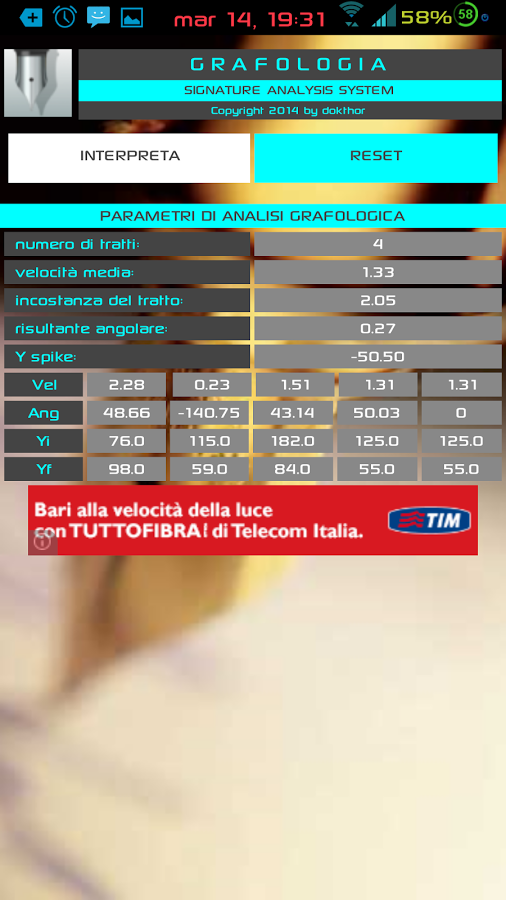
\includegraphics[height=0.5\textheight]{figures/analog_graphology_sign_analysis.png}
    \caption{<<GRAPHOLOGY signature analysis>>}
    \label{fig:domain:analog:graphology_sign_analysis}
\end{figure}

Основными возможностями ПС являются:
\begin{itemize}
  \item поддержка ОС Android;
  \item выполнение анализа без доступа в интернет;
  \item предоставление характеристик личности по 5 основным критериям.
\end{itemize}

Основными недостатками ПС являются:
\begin{itemize}
  \item поддержка только ОС Android;
  \item в разработке не участвовали эксперты графологи;
  \item механизм ввода подписи неочевиден;
  \item для ввода образцов почерка используется экран смартфона, что приводит к искажению в написании символов при низком разрешении и без использования стилуса.
\end{itemize}

\subsubsection{Graphology Lite}
\label{sub:domain:analogs:graphology_lite}

Программное средство <<Graphology Lite>> является приложением для операционной системы Android, разработанным компанией <<Hyperborea>>~\cite{analogs_graphology_lite}. Пользовательский интерфейс приложения представлен на рисунке~\ref{fig:domain:analogs:graphology_lite}.

\begin{figure}[h]
    \centering
    
\includegraphics[height=0.5\textheight]{figures/analog_graphology_lite.png}
    \caption{Программное средство <<Graphology Lite>>}
    \label{fig:domain:analogs:graphology_lite}
\end{figure}

Основными возможностями ПС являются:
\begin{itemize}
  \item поддержка ОС Android;
  \item выполнение анализа без доступа в интернет;
  \item использование для ввода экрана или фотографии почерка.
\end{itemize}

Основными недостатками ПС являются:
\begin{itemize}
  \item поддержка только ОС Android;
  \item в разработке не участвовали эксперты графологи;
  \item бесплатная версия позволяет произвести анализ только одного образца (платная версия стоит 1.05 \$).
\end{itemize}

В результате анализа было выявлено, что текущие аналоги, описанные в данном разделе, не обладают следующими возможностями, необходимыми для эффективного практического использования:
\begin{itemize}
  \item поддержка ОС Linux и MacOS;
  \item поддержка русского языка интерфейса;
  \item взимание платы за использование;
  \item поддержка механизма контроля доступа.
\end{itemize}

\todo[inline]{Описать что для разных уровней необходимо различный уровень детализации параметров (Расстояния между строками и словами нужно только в графологии)}
\subsection{Анализ литературных источников}
\label{sub:domain:literary_sources}

\todo[inline]{Добавить источники}
\subsubsection{Аутентификация на основе рукописной подписи}
Существуют два основных подхода к обработке рукописных образцов:
\begin{enumerate}
  \item Анализ самой подписи (подход сводится к сопоставлению двух изображений).
  \item Анализ характеристик подписи, средней силы нажима, скорости, ускорения, т.е. свертка, в которую входит информация по подписи, временными и статистическими характеристиками её написания~\cite{bryxomickii}.
\end{enumerate}

Первый подход отличается высокой скоростью работы, однако подвержен большему числу ошибок в связи с естественными отличиями в написании подписи из-за человеческой физиологии.
Второй подход обладает высокой точностью~\cite{nelson_kishon}, но требует существенных вычислительных затрат как на этапе предобработки образцов почерка и формирования эталонного образца, так и на этапе сопоставления образца, предъявляемого системе с эталонным.
Набор разработанных на сегодняшний день способов представления образцов почерка достаточно широк~\cite{ivanov_korparate_network}:
\begin{itemize}
  \item частотно-временное оконное преобразование Фурье;
  \item вейвлет-преобразование с радиальным базисом;
  \item локальные экстремумы;
  \item временные и статистические характеристики (скорость, нажим);
  \item эллипсы инерции.
\end{itemize}

Все вышеперечисленные методы можно условно разделить на группы по трактовке подпись, так, например, способ вейвлет-преобразование рассматривает подпись как цифровой сигнал, локальные экстремумы как функцию, а эллипсы инерции как физический объект. Методы, относящиеся к одной группе, имеют схожие достоинства и недостатки.
Основная сложность заключается в формировании списка признаков, которые, во-первых, будут уникально характеризовать любого пользователя, т.е. отрицать существование двух пользователей с одинаковыми значениями параметров, в-третьих значения признака не должно завесить от времени.

\subsubsection{Графология}
Публикации и научные статьи на темы схожие с темой данной работы можно условно разделить по следующим признакам:
\begin{itemize}
  \item метод сегментации изображения;
  \item метод классификации признаков изображения.
\end{itemize}

Метод сегментации изображения является неотъемлемой частью алгоритмов обработки рукописного текста, будь это распознавание или анализ. От качества сегментации напрямую зависит качество работы всего алгоритма поэтому выбор метода сегментации является важным этапом.

В рассмотренной литературе предлагаются следующие алгоритмы сегментации рукописного текста:
\begin{itemize}
  \item преобразования Хафа~\cite{louloudis_gatos_pratikakis_halatsis};
  \item нечеткие интервалы~\cite{louloudis_gatos_pratikakis_halatsis};
  \item нечеткий и адаптивный рекурсивный метод наименьших \mbox{квадратов~\cite{louloudis_gatos_pratikakis_halatsis};}
  \item статистические методы (средний интервал между строками)~\cite{gomathi_umadevi_mohanavel};
  \item метод Лоулодиса-Гатоса-Пратикакиса-Халатсиса (LGPH)~\cite{louloudis_gatos_pratikakis_halatsis};
  \item проецирование контуров~\cite{louloudis_gatos_pratikakis_halatsis}.
\end{itemize}

Преобразования Хафа являются мощным инструментом компьютерного зрения, позволяющим извлекать элементы из изображения. Данный метод позволяет достичь высокой точности сегментации текста, однако требует больших вычислительных затрат в связи с объемом вычислений и использованием тригонометрических функций при вычислении.

Метод рекурсивных нечетких и адаптивных наименьших квадратов, так же как и преобразования Хафа, широко используется для выделения областей изображения благодаря высокому качеству работы и устойчивости к шумам и искажениям, однако вычислительная стоимость данных методов относительно велика.

Метод Лоулодиса-Гатоса-Пратикакиса-Халатсиса показывает очень хорошие результаты сегментации и по результатам исследований превосходит по качеству и времени работы все приведенные выше алгоритмы, однако он пока находится в состоянии исследования и не имеет реальных примеров реализации и использования в практических проектах.

Методы проецирования контуров и нечетких интервалов хорошо подходят для распознавания печатного текста, но дают плохие результаты при распознавании рукописного из-за динамически изменяющихся интервалов между символами,строками и словами.

Статические методы основаны на разбиении изображении в зависимости от распределения средней яркости частей изображения, качества работы данных методов ниже чем у преобразований Хафа или рекурсивных методов на основе наименьших квадратов, но время работы намного меньше благодаря меньшему количеству вычислений и быстрым операциям сложению и делению.

В разрабатываемом программном средстве не требуется высокая точность распознавания, как например для распознавания текста, в то время как программное средство может работать с большим количеством изображений одновременно и быстродействие важно. Исходя из этого в качестве алгоритма сегментации будет использоваться статический метод.

Не менее важным является алгоритм классификации, так как именно он будет устанавливать соответствие между параметрами текста и психологическими характеристиками, например силой нажима и степенью наклона символа.

В рассмотренной литературе предлагаются следующие алгоритмы классификации признаков рукописного текста:
\begin{itemize}
  \item нейронные сети~\cite{champa_ananda_kumar_ann, grewal_prashar, gabrani_solomon_dviwe,puri_lakhwani, dang_kumar, kathait_singh};
  \item мешок особенностей~\cite{rothacker_bag_of_features};
  \item метод опорных векторов~\cite{slideshare_khandelwal_garg, gabrani_solomon_dviwe, prasad_singh_sapre};
  \item метод основанный на правилах~\cite{champa_ananda_kumar_rule_base}.
\end{itemize}

Метод основанный на правилах заключается в последовательной проверке соответствия параметров почерка набору правил <<если"=то>>. Как пример можно привести правило <<Если строки наклонены влево и сила нажима слабая, то человек пессимист не склонный к выражению эмоций>>. Данный подход основан только на описании графологических метод, обладает высокой скоростью и не требует обучения. Однако требуется определение границ значений анализируемых параметров, а так же количество правил экспоненциально растет с количеством параметров и их возможных значений, так для двух параметров с тремя значениями каждого понадобиться 9 правил~\cite{champa_ananda_kumar_rule_base}, а для пяти параметров уже 243.

Метод основанный на <<мешке особенностей>> состоит в составлении <<словаря слов>> на основе большой базы изображений. Данный словарь будет содержать фрагмент изображения описанный каким-либо дескриптором, например SIFT, и частоту появления этого фрагмента. По сути данный метод рассматривает задачу определения психологических параметров как задачу категоризации. Основными недостатками данного метода является необходимость в сборе и ручной обработке, определения параметров личности экспертами графологами, огромной базы изображений, т.к. все образцы почерка достаточно похожи и сложно выделить отличительные признаки.

Использование нейронных сетей является хорошим решением благодаря способности сети обобщать данные, а использование обратного распространения ошибок позволяет добиться очень хорошего качества распознавания. Однако выбор оптимальной структуры сети и функции активации нейронов является нетривиальной задачей, так же время обучения и распознавания относительно велико.

Метод опорных векторов основан на нахождении границы классов максимально удаленной от их экземпляров. К его достоинствам относиться хорошее качество распознавания, высокая скорость обучения и классификации. Однако необходим большой объем обучающей выборки, такой чтобы каждый из возможных наборов признаков встречался хотя бы раз. Так же вопрос выбора оптимального типа ядер схож с выбором функции активации для нейронных сетей.

Каждая из описанных задач имеет свои требования к детализации и сложности модели.

\todo[inline]{Описать методы Микрографии}
\todo[inline]{Описать методы аутентификации}

\todo[inline]{Описать типы устройств и форматов входных данных и их минусы дороговизна для спец сканеров, точность и неодходимость доп обработки и сегментации для изображений}
Применительно в задачам биометрической классификации так же используется разложение в ряд Фурье

Основываясь на проведенном анализе и объеме обучающей выборки, ($\sim$ 1500 образцов), было принято решение использовать метод опорных векторов в качестве классификатора. Точность классификации нейронных сетей и метода опорных векторов примерно равны, однако скорость обучения и распознавания у опорных векторов выше, что так же повлияло на решение.

\todo[inline]{Просмотреть раздел про технологии и системные требования}
\subsection{Обоснование выбора языка и сред разработки}
\label{sec:techs:intro}
Выбор технологий является важным предварительным этапом разработки сложных информационных систем. Платформа и язык программирования, на котором будет реализована система, заслуживает большого внимания, так как множество исследований показали, что выбор языка программирования значительно влияет на производительность труда программистов и качество создаваемого ими кода~\cite[c.~59]{mcconnell_2005}.

На выбор технологий повлияли следующие факторы:
\begin{itemize}
  \item программное средство должно быть выполнено в виде клиент"=серверного приложения;
  \item разрабатываемое ПО должно работать на операционных системах Linux, MacOS и Windows;
  \item разработчик имеет опыт работы с объектно"=ориентированными и функциональными языками программирования.
\end{itemize}

\subsubsection{Язык программирования Scala}
\label{sub:techs:scala}
Scala – мультипарадигмальный, компилируемый, строго типизированный язык программирования, спроектированный кратким и безопасным для простого и быстрого создания компонентного программного обеспечения, сочетающий возможности функционального и объектно-ориентированного программирования~\cite{wiki_scala}.

Scala поддерживает объектно-ориентированную и функциональную парадигмы программирования, но доминирующей является объектно-ориентированная. Язык был выпущен для общего пользования на платформе JVM и .NET, так же создан LLVM-компилятор (Scala Native) и транслятор в JavaScript (ScalaJS).

Отличительные особенности языка Scala:
\begin{itemize}
  \item Лаконичность. Код на Scala в средней вдвое короче кода на Java.
  \item Открытый исходный код. Код стандартной библиотеки опубликован к открытом доступе на портале GitHub и любой желающий, при наличии желания и способностей, может стать участником проекта.
  \item Высокий уровень абстракции. В стандартной библиотеке реализованы большинство типичных операции над строками и коллекциями, в частности итерация по элементам коллекции инкапсулирована в методах map, filter, flatMap. Так же выражение for трансформируется в вызов выше описанных методов, что позволяет использовать в нем пользовательские контейнеры и типы данных.
  \item Платформонезависимость. Код языка компилируется в JVM байт-код и может исполняться на любой платформе поддерживающей JVM.
  \item Строгая система типов. Позволяет выявить многое ошибки еще на стадии компиляции.
  \item Объектно-ориентированность. Язык поддерживает основные концепции объектно-ориентированного программирование (наследование, инкапсуляция, полиморфизм).
  \item Функциональность. Язык поддерживает основные концепции функционального программирование (функции высших порядков, сопоставление с образцов, <<ленивые>> вычисления).
  \item Расширяемость. В языке присутствуют механизм (неявные преобразования) позволяющий расширять функционал стандартных классов и сторонних библиотек.
  \item Использование Java-кода. Возможно использовать не только библиотеки написанные на Java, но и классы написанные на Java в Scala-проекте, но отсутствует полная обратная совместимость.
  \item Широкий набор библиотеки. Стандартная библиотека Scala содержит классы для работы с вводом-выводом, регулярными выражениями, параллельной обработки, работы со строками, коллекции. Так же существует большое количество сторонних библиотек.
\end{itemize}

\paragraph{Объектно-ориентированное программирование}
Объектно-ориентированная парадигма программирования играет в языке важную роль. Стандартная библиотека языка реализована в виде набора классов и примесей, а так же модульность обеспечивается классами и пакетами~\cite{horsman_scala}.

Особенности Scala с точки зрения объектно"=ориентированной \mbox{парадигмы:}
\begin{itemize}
  \item статическая сильная полная типизация с автоматическим \mbox{выведением типов;}
  \item наследование, в том числе использование примесей (Traits);
  \item полиморфизм;
  \item инкапсуляция;
  \item конструкторы, деструкторы;
  \item все математические операторы являются методами;
  \item гибкое управление доступом к полям и методам;
  \item метапрограммирование;
  \item объекты компаньоны (используются для инкапсуляции статических полей и методов).
\end{itemize}

\paragraph{Функциональное программирование}
Особенности Scala с точки зрения функциональной парадигмы:
\begin{itemize}
  \item функции высших порядков;
  \item функции объект первого класса;
  \item оптимизация хвостовой рекурсии;
  \item сопоставление с образцов;
  \item поддержка неизменяемых структур данных;
  \item функциональные комбинаторы и композиции;
  \item частичное применение функции;
  \item <<ленивые>> вычисления;
  \item структурное переиспользование неизменяемых коллекций.
\end{itemize}

Основываясь на выше перечисленных факторах было принято решение использовать в качестве основного языка программирования Scala как современный, активно набирающий популярность язык, поддерживающий функциональную и объектно"=ориентированную парадигмы программирования. Так же благодаря интеграции с Java, части кода требующего быстродействия могут быть реализованы на этом языке.

\subsubsection{Фреймворк Akka}
\label{sec:techs:akka}

Akka – набор прикладных библиотек (фреймворк) предоставляющий высокоуровневый интерфейс для разработки, развертывания и отладки систем акторов.

Основными достоинствами фреймворка Akka являются:
\begin{itemize}
  \item Простота интерфейса, высокая степень абстракции.
  \item Устойчивость к отказам, благодаря механизму супервизор.
  \item Масштабируемость. Простата добавления акторов в систему и развертывания компонентов на другой машине.
  \item Высокая скорость работы и степень параллелизма, благодаря использованию модели акторов;
  \item Минимально количество блокирующих операций, отсутствие общего изменяемого состояния.
\end{itemize}

\begin{figure}[ht]
    \centering
    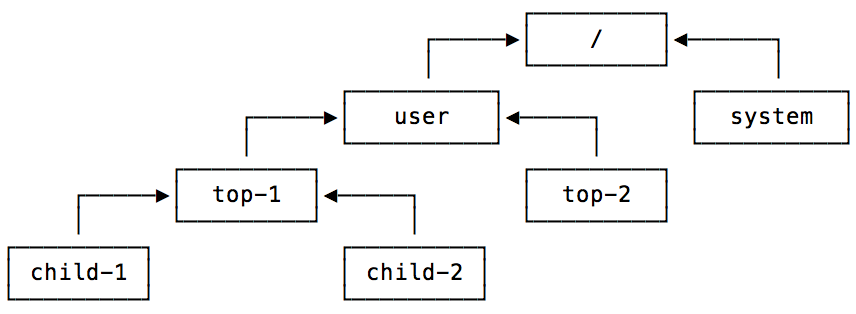
\includegraphics[width=0.7\textwidth]{figures/actors_hier.png}
    \caption{Иерархия акторов}
    \label{fig:techs:akka:actor_hierar}
\end{figure}

\paragraph{Модель акторов}
\label{sec:techs:akka:actor_model}
Модель акторов - модель параллельных вычислений, основанная на взаимодействии изолированных примитивов, взаимодействующих по средствам получения и отправки сообщений. Впервые была предложена в 1973 году~\cite{hewitt_bishop_steiger_actor_model}.

Основным понятием данной модели является «актор». Согласно модели актор лишен состояния и информации о структуре системы (количество братьев и родителей).

На рисунке~\ref{fig:techs:akka:actor_hierar} представлена иерархия акторов, в данном случае <<top-1>> является родителем для акторов <<child-1>> и <<child-2>>. Актор <<top-1>> выполняет функции супервизора и в случае ошибки в дочерних акторах получает соответствущее сообщение и может принимать решение для его исправлению, например перезапустить актор. Так же в случае необходимости можно делегировать принятие решения родительскому актору, в данном примере <<user>>.
\begin{figure}[ht]
    \centering
    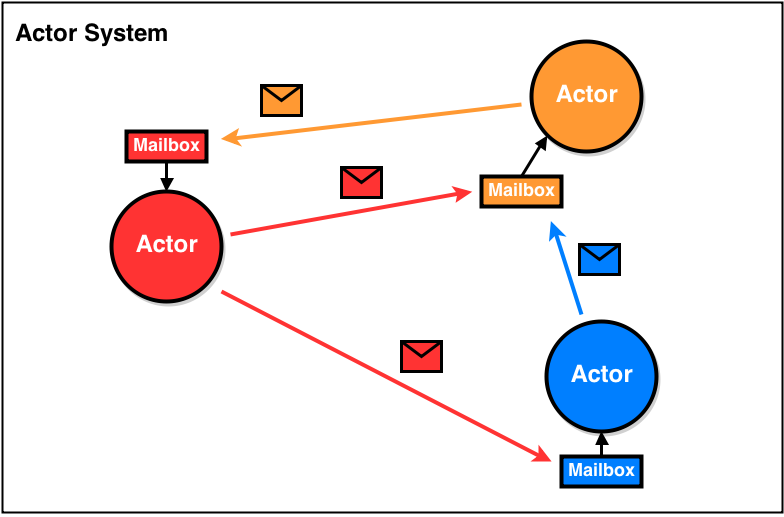
\includegraphics[width=0.7\textwidth]{figures/actor_model.png}
    \caption{Пример взаимодействия акторов}
    \label{fig:techs:akka:actor_model:comulication}
\end{figure}

Как видно на рисунке~\ref{fig:techs:akka:actor_model:comulication}, отсутствует прямое взаимодействия акторов между собой, вся коммуникация осуществляется при помощи передачи сообщений. В совокупности с использованием неизменяемых структур данных, механизм сообщений делает всю работу системы акторов априорно асинхронной и неблокирующей.

При получении сообщения актор может:
\begin{itemize}
  \item отправить конечное число сообщений другим акторам;
  \item создать конечное число новых акторов;
  \item выбрать поведение, которое будет использоваться при обработке следующего полученного сообщения.
\end{itemize}

Данный подход позволяет теоретически полностью избежать блокировок благодаря отсутствию прямых вызовов методов актора и даже механизма ожидания ответа, позволяет добиться прироста производительности сопоставимого с количеством ядер процессоров в среде исполнения, чего невозможно добиться при использовании классической модели параллельности на основе потоков и блокировках при доступе к общему изменяемому состоянию.

Перечисленные достоинства, в особенности устойчивой к отказам и простота масштабирования, являются крайне важными при реализации архитектуры на основе микросервисов. Исходя из выше перечисленного, для обеспечения параллельной обработки данных будет использоваться набор прикладных библиотек (фреймворк) Akka.

\subsubsection{Фреймворк Akka Http}
\label{sec:techs:spray}

Akka-Http – набор прикладных библиотек (фреймворк), предназначенный для реализации веб-приложений, написанный на Scala. Фреймворк базируется на описанном выше фреймворке Akka и реализует асинхронное распределение запросов пользователя на иерархию акторов. Является наследником фремворка Spray и копирует его основные концепции и компоненты.

Основными достоинствами фреймворка Akka Http являются:
\begin{itemize}
  \item полная асинхронность, отсутствие блокировок (весь интерфейс полностью асинхронный);
  \item высокая производительность (используются специальные низкоуровневые компоненты);
  \item модульность (весь интерфейс полностью асинхронный);
  \item легковесность (включаются только необходимые модули).
\end{itemize}

Данный набор библиотек достаточно молодой и еще не получил широкого распространения в коммерческой разработке, что может сказаться на стабильности работы и производительности, однако разработчики быстро устраняют дефекты и выпускают новые версии фреймворка раз в месяц. Использование данного фреймворка позволит упростить и ускорить разработку, отладку и последующее сопровождения благодаря использования одной концепции с предыдущим фреймворком.
Альтернативой является использование таких фреймворком как Lift и Play, однако они не имеют встроенной поддержки модели акторов, а так же требует дополнительных компонентов, контейнера Сервлетов, например Tomcat или Jetty, для развертывания.

Исходя из выше перечисленного, для реализации серверной части приложения будет использоваться набор прикладных библиотек Akka Http, так как несмотря на возможные недоработки он хорошо встраивается в экосистему данной работы.

\subsubsection{Библиотека TensorFlow}
\label{sec:techs:tensor_flow}
\emph{TensorFlow} — открытая программная библиотека для машинного обучения, разработанная компанией Google для решения задач построения и тренировки нейронной сети с целью автоматического нахождения и классификации образов, достигая качества человеческого восприятия Применяется как для исследований, так и для разработки собственных продуктов Google. Основное API для работы с библиотекой реализовано для Python, также существуют реализации для C++, Haskell, Java, Go и Swift.

Является продолжением закрытого проекта DistBelief. Изначально TensorFlow была разработана командой Google Brain для внутреннего использования в Google, в 2015 году система была переведена в свободный доступ с открытой лицензией Apache 2.0.

\subsection{Постановка задачи}
\label{sec:domain:requirements}
В результате выполнения диссертационной работы должно быть разработано программное средство определения психологических параметров личности по образцу почерка, реализующее процедуры выделения признаков почерка из изображения и их классификацию, а так же механизм авторизации для обеспечения секретности данных.

Разрабатываемое программное средство должно выполнять следующие функции:
\begin{itemize}
  \item регистрация пользователя;
  \item авторизация пользователя;
  \item просмотр сохраненных образцов почерка;
  \item удаление сохраненных образцов почерка;
  \item добавление нового образца почерка;
  \item выделение признаков образца почерка;
  \item определение психологических характеристик личности;
  \item определение неврологических отклонений;
  \item проведение биометрической аутентификации.
\end{itemize}

К разрабатываемому программному средству предъявляются следующие требования:
\begin{itemize}
  \item разрабатываемое ПО должно работать на операционных системах Linux, MacOS и Windows;
  \item модуль программного средства требует 512 MB оперативной памяти;
  \item программное средство должно быть выполнено в виде клиент"=серверного приложения;
  \item программное средство должно поддерживать русский язык \mbox{интерфейса;}
  \item выходными данными являются документы в формате JSON описывающий результаты анализа образца почерка;
  \item входными данными являются документы в формате JSON описывающий координаты точек образца почерка.
\end{itemize}